%  LaTeX support: latex@mdpi.com 
%  For support, please attach all files needed for compiling as well as the log file, and specify your operating system, LaTeX version, and LaTeX editor.

%=================================================================
\documentclass[journal,article,submit,pdftex,moreauthors]{Definitions/mdpi} 
% For posting an early version of this manuscript as a preprint, you may use "preprints" as the journal and change "submit" to "accept". The document class line would be, e.g., \documentclass[preprints,article,accept,moreauthors,pdftex]{mdpi}. This is especially recommended for submission to arXiv, where line numbers should be removed before posting. For preprints.org, the editorial staff will make this change immediately prior to posting.

%--------------------
% Class Options:
%--------------------
%----------
% journal
%----------
% Choose between the following MDPI journals:
% acoustics, actuators, addictions, admsci, adolescents, aerospace, agriculture, agriengineering, agronomy, ai, algorithms, allergies, alloys, analytica, animals, antibiotics, antibodies, antioxidants, applbiosci, appliedchem, appliedmath, applmech, applmicrobiol, applnano, applsci, aquacj, architecture, arts, asc, asi, astronomy, atmosphere, atoms, audiolres, automation, axioms, bacteria, batteries, bdcc, behavsci, beverages, biochem, bioengineering, biologics, biology, biomass, biomechanics, biomed, biomedicines, biomedinformatics, biomimetics, biomolecules, biophysica, biosensors, biotech, birds, bloods, blsf, brainsci, breath, buildings, businesses, cancers, carbon, cardiogenetics, catalysts, cells, ceramics, challenges, chemengineering, chemistry, chemosensors, chemproc, children, chips, cimb, civileng, cleantechnol, climate, clinpract, clockssleep, cmd, coasts, coatings, colloids, colorants, commodities, compounds, computation, computers, condensedmatter, conservation, constrmater, cosmetics, covid, crops, cryptography, crystals, csmf, ctn, curroncol, currophthalmol, cyber, dairy, data, dentistry, dermato, dermatopathology, designs, diabetology, diagnostics, dietetics, digital, disabilities, diseases, diversity, dna, drones, dynamics, earth, ebj, ecologies, econometrics, economies, education, ejihpe, electricity, electrochem, electronicmat, electronics, encyclopedia, endocrines, energies, eng, engproc, ent, entomology, entropy, environments, environsciproc, epidemiologia, epigenomes, est, fermentation, fibers, fintech, fire, fishes, fluids, foods, forecasting, forensicsci, forests, foundations, fractalfract, fuels, futureinternet, futureparasites, futurepharmacol, futurephys, futuretransp, galaxies, games, gases, gastroent, gastrointestdisord, gels, genealogy, genes, geographies, geohazards, geomatics, geosciences, geotechnics, geriatrics, hazardousmatters, healthcare, hearts, hemato, heritage, highthroughput, histories, horticulturae, humanities, humans, hydrobiology, hydrogen, hydrology, hygiene, idr, ijerph, ijfs, ijgi, ijms, ijns, ijtm, ijtpp, immuno, informatics, information, infrastructures, inorganics, insects, instruments, inventions, iot, j, jal, jcdd, jcm, jcp, jcs, jdb, jeta, jfb, jfmk, jimaging, jintelligence, jlpea, jmmp, jmp, jmse, jne, jnt, jof, joitmc, jor, journalmedia, jox, jpm, jrfm, jsan, jtaer, jzbg, kidney, kidneydial, knowledge, land, languages, laws, life, liquids, literature, livers, logics, logistics, lubricants, lymphatics, machines, macromol, magnetism, magnetochemistry, make, marinedrugs, materials, materproc, mathematics, mca, measurements, medicina, medicines, medsci, membranes, merits, metabolites, metals, meteorology, methane, metrology, micro, microarrays, microbiolres, micromachines, microorganisms, microplastics, minerals, mining, modelling, molbank, molecules, mps, msf, mti, muscles, nanoenergyadv, nanomanufacturing, nanomaterials, ncrna, network, neuroglia, neurolint, neurosci, nitrogen, notspecified, nri, nursrep, nutraceuticals, nutrients, obesities, oceans, ohbm, onco, oncopathology, optics, oral, organics, organoids, osteology, oxygen, parasites, parasitologia, particles, pathogens, pathophysiology, pediatrrep, pharmaceuticals, pharmaceutics, pharmacoepidemiology, pharmacy, philosophies, photochem, photonics, phycology, physchem, physics, physiologia, plants, plasma, pollutants, polymers, polysaccharides, poultry, powders, preprints, proceedings, processes, prosthesis, proteomes, psf, psych, psychiatryint, psychoactives, publications, quantumrep, quaternary, qubs, radiation, reactions, recycling, regeneration, religions, remotesensing, reports, reprodmed, resources, rheumato, risks, robotics, ruminants, safety, sci, scipharm, seeds, sensors, separations, sexes, signals, sinusitis, skins, smartcities, sna, societies, socsci, software, soilsystems, solar, solids, sports, standards, stats, stresses, surfaces, surgeries, suschem, sustainability, symmetry, synbio, systems, taxonomy, technologies, telecom, test, textiles, thalassrep, thermo, tomography, tourismhosp, toxics, toxins, transplantology, transportation, traumacare, traumas, tropicalmed, universe, urbansci, uro, vaccines, vehicles, venereology, vetsci, vibration, viruses, vision, waste, water, wem, wevj, wind, women, world, youth, zoonoticdis 

%---------
% article
%---------
% The default type of manuscript is "article", but can be replaced by: 
% abstract, addendum, article, book, bookreview, briefreport, casereport, comment, commentary, communication, conferenceproceedings, correction, conferencereport, entry, expressionofconcern, extendedabstract, datadescriptor, editorial, essay, erratum, hypothesis, interestingimage, obituary, opinion, projectreport, reply, retraction, review, perspective, protocol, shortnote, studyprotocol, systematicreview, supfile, technicalnote, viewpoint, guidelines, registeredreport, tutorial
% supfile = supplementary materials

%----------
% submit
%----------
% The class option "submit" will be changed to "accept" by the Editorial Office when the paper is accepted. This will only make changes to the frontpage (e.g., the logo of the journal will get visible), the headings, and the copyright information. Also, line numbering will be removed. Journal info and pagination for accepted papers will also be assigned by the Editorial Office.

%------------------
% moreauthors
%------------------
% If there is only one author the class option oneauthor should be used. Otherwise use the class option moreauthors.

%---------
% pdftex
%---------
% The option pdftex is for use with pdfLaTeX. If eps figures are used, remove the option pdftex and use LaTeX and dvi2pdf.

%=================================================================
% MDPI internal commands
\usepackage{array}
\firstpage{1} 
\makeatletter 
\setcounter{page}{\@firstpage} 
\makeatother
\pubvolume{1}
\issuenum{1}
\articlenumber{0}
\pubyear{2022}
\copyrightyear{2022}
%\externaleditor{Academic Editor: Firstname Lastname}
\datereceived{} 
\dateaccepted{} 
\datepublished{} 
%\datecorrected{} % Corrected papers include a "Corrected: XXX" date in the original paper.
%\dateretracted{} % Corrected papers include a "Retracted: XXX" date in the original paper.
\hreflink{https://doi.org/} % If needed use \linebreak
%\doinum{}
%------------------------------------------------------------------
% The following line should be uncommented if the LaTeX file is uploaded to arXiv.org
%\pdfoutput=1

%=================================================================
% Add packages and commands here. The following packages are loaded in our class file: fontenc, inputenc, calc, indentfirst, fancyhdr, graphicx, epstopdf, lastpage, ifthen, lineno, float, amsmath, setspace, enumitem, mathpazo, booktabs, titlesec, etoolbox, tabto, xcolor, soul, multirow, microtype, tikz, totcount, changepage, attrib, upgreek, cleveref, amsthm, hyphenat, natbib, hyperref, footmisc, url, geometry, newfloat, caption

%=================================================================
%% Please use the following mathematics environments: Theorem, Lemma, Corollary, Proposition, Characterization, Property, Problem, Example, ExamplesandDefinitions, Hypothesis, Remark, Definition, Notation, Assumption
%% For proofs, please use the proof environment (the amsthm package is loaded by the MDPI class).

%=================================================================
% Full title of the paper (Capitalized)
\Title{Distributed location-aware task offloading in multi-UAVs enabled edge computing }

% MDPI internal command: Title for citation in the left column
\TitleCitation{Distributed location-aware task offloading in multi-UAVs enabled edge computing}

% Author Orchid ID: enter ID or remove command
\newcommand{\orcidauthorA}{0000-0002-4475-3608} % Add \orcidA{} behind the author's name
%\newcommand{\orcidauthorB}{0000-0000-0000-000X} % Add \orcidB{} behind the author's name

% Authors, for the paper (add full first names)
\Author{Jianhua Liu $^{1*}$\orcidA{},Zibo Wu $^{1}$,Jiajia Liu $^{1}$,Xiaoguang Tu $^{1}$}

%\longauthorlist{yes}

% MDPI internal command: Authors, for metadata in PDF
\AuthorNames{Firstname Lastname, Firstname Lastname and Firstname Lastname}

% MDPI internal command: Authors, for citation in the left column
\AuthorCitation{Lastname, F.; Lastname, F.; Lastname, F.}
% If this is a Chicago style journal: Lastname, Firstname, Firstname Lastname, and Firstname Lastname.

% Affiliations / Addresses (Add [1] after \address if there is only one affiliation.)
\address{%
$^{1}$ \quad Institute of Electronic and Electrical Engineering, Civil Aviation Flight University of China, Guanghan,Sichuan, 618307, China; jianhuacafuc13@cafuc.edu.cn(J.-L); lietiansha@sina.com(Z.-W); cafucljj@163.com(J.-L);xguangtt@hotmail.com(X.-T)}

% Contact information of the corresponding author
\corres{Correspondence: jianhuacafuc13@cafuc.edu.cn}

% Current address and/or shared authorship

% The commands \thirdnote{} till \eighthnote{} are available for further notes

%\simplesumm{} % Simple summary

%\conference{} % An extended version of a conference paper

% Abstract (Do not insert blank lines, i.e. \\) 
\abstract{Edge computing is a new computing paradigm which distributes tasks to edge networks for processing, it provides effective support for various mobile applications to meet their rapid response requirement.  Unmanned Aerial Vehicle (UAV) has been widely used in emergency rescue, mapping, etc., with the advantages of flexible deployment and rapid movement. However, on one hand, mobile applications will be terminated when the battery energy is exhausted. On the other hand, mobile applications will be out of service when mobile devices are out of radio coverage of UAVs. How to achieve low-cost task unloading in the resource limited and location sensitive multi-UAVs edge computing environment is rather challenging. In this paper, we propose a distributed location-aware task offloading  scheme, aiming at the  above issues. Specifically, we create a nonlinear task allocation problem by combining the limited energy constraints of edge nodes with the random movement of users, where the cost function is divided into  static and dynamic costs, respectively. Then, we formulate this problem to a convex optimization one with linear constrains, based on regularization technology. The mathematical proof shows that the scheme can support a parameterized competitive ratio without requiring any prior knowledge of the input task. The simulation results show that the proposed scheme can achieve lower cost edge computing services.} 

% Keywords
\keyword{edge computing; UAV; task allocation; convex programming}


% The fields PACS, MSC, and JEL may be left empty or commented out if not applicable
%\PACS{J0101}
%\MSC{}
%\JEL{}

%%%%%%%%%%%%%%%%%%%%%%%%%%%%%%%%%%%%%%%%%%
% Only for the journal Diversity
%\LSID{\url{http://}}

%%%%%%%%%%%%%%%%%%%%%%%%%%%%%%%%%%%%%%%%%%
% Only for the journal Applied Sciences:
%\featuredapplication{Authors are encouraged to provide a concise description of the specific application or a potential application of the work. This section is not mandatory.}
%%%%%%%%%%%%%%%%%%%%%%%%%%%%%%%%%%%%%%%%%%

%%%%%%%%%%%%%%%%%%%%%%%%%%%%%%%%%%%%%%%%%%
% Only for the journal Data:
%\dataset{DOI number or link to the deposited data set in cases where the data set is published or set to be published separately. If the data set is submitted and will be published as a supplement to this paper in the journal Data, this field will be filled by the editors of the journal. In this case, please make sure to submit the data set as a supplement when entering your manuscript into our manuscript editorial system.}

%\datasetlicense{license under which the data set is made available (CC0, CC-BY, CC-BY-SA, CC-BY-NC, etc.)}

%%%%%%%%%%%%%%%%%%%%%%%%%%%%%%%%%%%%%%%%%%
% Only for the journal Toxins
%\keycontribution{The breakthroughs or highlights of the manuscript. Authors can write one or two sentences to describe the most important part of the paper.}

%%%%%%%%%%%%%%%%%%%%%%%%%%%%%%%%%%%%%%%%%%
% Only for the journal Encyclopedia
%\encyclopediadef{Instead of the abstract}
%\entrylink{The Link to this entry published on the encyclopedia platform.}
%%%%%%%%%%%%%%%%%%%%%%%%%%%%%%%%%%%%%%%%%%
\begin{document}

%%%%%%%%%%%%%%%%%%%%%%%%%%%%%%%%%%%%%%%%%%
\setcounter{section}{-1} %% Remove this when starting to work on the template.
\section{Introduction}

Currently, with the development of communication and chip technologies, the Internet of Things (IoT) is outstanding in improving humans' quality of life. Users can quickly obtain information and process various tasks through the IoT. However, many IoT devices are subject to restrictions, such as limited storage and computation capacity, and imbalanced distribution of the capacity among these devices, which can reduce the service performance of the IoT. Cloud computing can enhance the IoT's capability in terms of storage, computation and management of various resources \cite{Shenshihao20,Salaht20,ShiWeisong16}. Unfortunately, because the cloud is far away from users, the response time of cloud computing can not meet real-time applications for IoT-based applictions. Edge computing is a new paradigm that aims to reduce the burden on Cloud and improve the response delay of requirements. With edge computing, many tasks can be completed directly by these edge computing devices without the participation of the cloud \cite{Liuyaqiong20}. To provide more flexible services, mobile edge computing (MEC) is proposed to enhance the information processing capabilities of mobile devices regardless of their high location sensitivity. However, these edge devices are often heterogeneous, their computing capacities are quite different, and there exists a competitive relationship among these edge devices, therefore, there are still some energy consumption and reliability problems with MEC that must be solved.

The MEC is vulnerable on reliability, especially high dynamics that frequently occur in UAV-enabled MEC. Unlike conventional Internet of Vehicles (IoV), the movement trajectory of a mobile node is predictable and always transforms along a certain road. Although existing computation offloading schemes are effective in achieving low latency for mobile users, for battery-powered UAVs, the computation performance may be compromised due to limited battery energy and radio coverage for task offloading. On one hand, mobile applications will be terminated when the battery energy is exhausted \cite{YuyiMao2016}. On the other hand, mobile applications will be out of service when mobile devices are out of radio coverage of UAVs. It is difficult to guarantee a robust edge computing service with minimum latency during rapid movement, especially if loT devices produce a lot of data that require processing in real-time \cite{Faraci20}. Besides the computation time cost, as discussed in \cite{XuY21,WangH19,ZhanC19,ZengY18}, UAV-enabled MEC in multi-UAVs environments incurs an additional time overhead on task migration from one UAV to another UAV since the UAV has limited computation capability. 

To solve the above problems, an multi-UAVs enabled edge computing scheme was proposed. Edge computing is performed at the Internet's edge with multiple UAVs. Edge  nodes also refers to cloudlets, and fog nodes, which has advantages in the quick response to IoT applications \cite{Wangtian19,Satyanarayanan17}. Motivated by \cite{WANG}, we divide the cost of task offloading into dynamic cost and static cost, these cost can be calculated by operating cost, QoS cost and Migration cost. The position changing of UAVs is an important factor affecting the task offloading strategy. In summary, the main contributions of
this work are presented as follows,


1. To solve the problem of dynamic task assignment in a UAV environment, a comprehensive optimization model is constructed. This model takes full account of the energy limit and location sensitivity of nodes,  can comprehensively optimize the migration cost, operation cost, and quality of service (QoS) cost.


2. The above problem is converted into a convex optimization problem, and an efficient online algorithm is proposed. Through rigorous competitive analysis, it is proved that the proposed algorithm has a parameterized competitive ratio.


3. The simulation results show that the proposed scheme has reliable robustness regardless of various numbers of users and UAV nodes, and can save $20\%$ of the total cost than other methods.






This paper is organized as follows. In Secion 1, related work is introduced. Section 2
describes our models and formulates the problem. Section 3 focuses on the design details of online algorithm. Section 4 presents the formal competitive analysis. Experiment results and analyses are reported in Section 5. The final section concludes this paper.

\section{Related Work}

Duo to the development of chip and communication technology, the popularity of mobile devices is growing rapidly, such as smart phones, wearable devices, smart cars, robots and UAVs. Edge Computing integrates resources to provide users with real-time and feasible service on the side of the Internet. Edge Computing releases the pressure on the cloud effectively and realizes the reliable utilization of optimized resource allocation on the edge Internet. A large number of location-sensitive mobile application services have grown rapidly because of the rapid development of Thing of Internet (IoT) and artificial intelligence (AI), such as intelligent maintenance, intelligent logistics, and so on. Unmanned aerial vehicle (UAV) has the advantages of flexible deployment and rapid movement. It is widely used in emergency rescue, aerial photography, logistics, and so on. In addition, the wireless communication channel between UAV and ground equipment has strong line-of-sight characteristics \cite{WU Q}, which could provide high quantity communication services and edge computing services for users. UAV edge computing platform supplies fast and flexible information support for mobile services. Researchers pay more attention that Multi-UAVs could cover a wider testing scale in recent years\cite{CUI G F,JI J,WANG Y P}.

The main problem for edge computing is how to provide a dynamic task assignment scheme for various mobile applications in a distributed environment \cite{GOPIKA P,PAN J L,ZHANG K Y,ZHANG N,WANG S,LIU}. Because edge cloud is heterogeneous and dynamic, neither resource allocation scheme nor task offloading scheme is suitable for the large-scale central cloud. The user location is mobility-agnostic, and the task scheduling of edge cloud can not be one-off, but an adaptive scheme that changes with the user's location. Therefore, the cost of task offloading is also an adaptive cost, including bandwidth cost, migration cost, latency cost, and so on\cite{WANG}.

A resource allocation scheme based on convex programming was proposed in \cite{WANG} to decrease the service cost for edge computing, optimizing operation cost, migration cost, and reconfiguration cost. Unfortunately, this scheme ignored the energy limit of mobile edge nodes. A task assignment model based on hybrid nonlinear programming \cite{HABER} was constructed  to reduce service delay in the ultra-dense software defined network (SDN)and saved energy consumption of edge cloud users. Under the condition of time latency constraint, joint optimization was used to minimize the sum of energy consumption of local devices, to obtain a computing offloading scheme based on energy efficiency under a single MEC node. However, this scheme only considered a single edge node and did not discuss the mobility of nodes, so the scope of application was limited. A  task assignment scheme was proposed in \cite{CHEN M}, which could reduce the task execution delay and improve the data transmission rate. The scheme reduced the delay of edge service and provided security protection for the information being processed. To enhance the privacy of users, Puthal et al. \cite{PUTHAL} proposed a service allocation scheme based on trust awareness, which was a multi-objective optimization scheme based on privacy entropy, energy consumption, and delay. Unfortunately, the scheme ignored the user's energy consumption limitation and mobility. To guarantee the fairness of different edge devices in a completely distributed environment, Xu et al. \cite{XU X L} applied simulation learning to resource scheduling algorithm of edge computing, and realized the transformation from local optimal solution to global optimal solution by guiding the online training of multi-agents with simulation learning results of multiple experts. But the convergence of the algorithm was not discussed in this work. To solve the problem of passive eavesdropping on the ground when ground users offload data to the edge computing network of multi-UAVs, Cui et al. \cite{CUI G F} proposed a safe task offloading strategy to minimize system energy consumption through joint optimization between user and resource, but this scheme ignored the position sensitivity of UAVs. By taking into consideration the inter-dependencies of the tasks, dynamic network states, and energy constraints of the UAVs, \cite{Zhusc20} formulate the average mission response time minimization problem and then model it as a Markov decision process. To achieve optimal average delay over trajectory, an edge computing framwork \cite{Callegaro2021} was developed which allowed enabling optimal offloading decisions as a function of network, computation load parameters and current state. The optimization is formulated as an optimal stopping time problem over a semi-Markov process. To maximize the secure computation efficiency, a two-stage alternative optimization algorithm \cite{Amos2021} was  proposed  by jointly optimizing the transmission power and UAV's trajectory. 

Unfortunately, the efficiency of these schemes for large task volume is questionable since they ignored the queuing time of tasks in a high dynamic environment. Moreover, few studies consider the rapid movement together with battery capacity limitation. Different from the above literatures, our paper proposes a dynamic task offloading scheme and exploits 
optimizing the online task offloading of IoT applications for the MEC network.



%\endnote{This is an endnote.} % To use endnotes, please un-comment \printendnotes below (before References). Only journal Laws uses \footnote.

% The order of the section titles is: Introduction, Materials and Methods, Results, Discussion, Conclusions for these journals: aerospace,algorithms,antibodies,antioxidants,atmosphere,axioms,biomedicines,carbon,crystals,designs,diagnostics,environments,fermentation,fluids,forests,fractalfract,informatics,information,inventions,jfmk,jrfm,lubricants,neonatalscreening,neuroglia,particles,pharmaceutics,polymers,processes,technologies,viruses,vision


@article{ID,
	author = {author},
	title = {title},
	journaltitle = {journaltitle},
	date = {date},
	OPTtranslator = {translator},
	OPTannotator = {annotator},
	OPTcommentator = {commentator},
	OPTsubtitle = {subtitle},
	OPTtitleaddon = {titleaddon},
	OPTeditor = {editor},
	OPTeditora = {editora},
	OPTeditorb = {editorb},
	OPTeditorc = {editorc},
	OPTjournalsubtitle = {journalsubtitle},
	OPTissuetitle = {issuetitle},
	OPTissuesubtitle = {issuesubtitle},
	OPTlanguage = {language},
	OPToriglanguage = {origlanguage},
	OPTseries = {series},
	OPTvolume = {volume},
	OPTnumber = {number},
	OPTeid = {eid},
	OPTissue = {issue},
	OPTmonth = {month},
	OPTpages = {pages},
	OPTversion = {version},
	OPTnote = {note},
	OPTissn = {issn},
	OPTaddendum = {addendum},
	OPTpubstate = {pubstate},
	OPTdoi = {doi},
	OPTeprint = {eprint},
	OPTeprintclass = {eprintclass},
	OPTeprinttype = {eprinttype},
	OPTurl = {url},
	OPTurldate = {urldate},
}
\section{System Model and Problem Description}
\subsection{System model}
Weconsider a time-slotted system whose whole running time $T$ is divided into $h$ time slots, and denote $T=\{t_1,t_2,\dots,t_h\}$, $(h \in Z^+)$. We envisage an edge computing system with $m$ users, denoted by $U=\{u_1,u_2,\dots,u_m\}$,($m \in Z^+$). We consider an edge-compatible mobile service where a set of  $n$ UAV edge nodes,  denoted by $S=\{s_1,s_2,\dots,s_n\}$, ($n \in Z^+$). The $m$ users and $n$ UAVs are distributed in the considered area  and their locations changes randomly at time slot $t_i(1 \le i \le h)$. The maximum data processing power of edge cloud is denoted by $C_s, s\in S$. The internet transforming latency between two edge nodes $s_1$ and $s_2$ is denoted by  $d(s_1,s_2)\ge 0$,  $\forall s\in S$, $d(s,s)=0$ is feasible. Each edge node  can cover a certain area. Each user can choose the closest edge node with the best transmission effect to establish transmission link and upload workloads. 

Since the position of UAVs and the users changes randomly at each time slot $t$, the links of the users in the system also change randomly. We assume that the transmission link established by the user is stable and remains unchanged at a time slot $t_i(1 \le i \le h)$. $l_{u,t}$ indicates the position of user $u$ at time slot $t \in T$. $s_{u,t}^{*}$ indicates that user $u$ establishes a transmission link with edge node $s$ at time slot $t\in T$, and $u$ offloads her tasks to the edge node $s$. $x_{u,s,t}$ represents the amount of tasks that user $u$ offloads to edge node $s$ at time slot $t$. We denote the total number of tasks by $\lambda_u$. The data processing capability of $s$ at time slot $t$ is denoted by $q_{s,t}$.   

 Table~\ref{tab2} shows the correspondent relationship between words and~abbreviations.

 The architecture of our proposed multi-UAVs enabled MEC system is shown in Fig.1. The system consists of a number of IoT applications, UAVs, base stations, cloud, wireless connections between UAV and IoT applications, and transmission links between UAVs, and transmission links between UAV and base station. IoT applications are usually pinned on some IoT nodes, such as smart phone, camera, Raspberry Pi and other sensors. The IoT applications can obtain a large amount of first-hand data from application environments such as earthquake, tsunami and smart farm, then transmit these data to the nearest UAV for further processing. When an UAV flies over these mobile applications, these applications will upload data processing tasks to the UAV. Based on the requirements of real-time and  cost management, the UAV may  divide the tasks into multiple subtasks and transmit the subtasks to other UAVs for processing. Therefore,  task offloading  is not a one-shot task and needs to be continuously adapted to accommodate UAVs' and applications' movements, incurring the “adaptation cost” over time. Every application and UAV can move arbitrarily in the system, and, from a time-slotted view, an application may connect to the UAV in one time slot and switch to another in the next. In each time slot the system can have its own optimal task allocation strategy, which may, however, become suboptimal if the adaptation cost during time-slot transition is considered. 

In this paper, we mainly focus on the task allocation in the edge network equipped with multi-UAVs, ignore the situation that the UAV sends the task to cloud for processing. It is assumed that each UAV is equipped with a directional  antenna to receive data from IoT applications and two transmit antenna systems for data transmission. Note that the UAV may suffer from the influences of aerodynamic forces. In order to guarante  the stability of signals transmitted in our system, we assume that the antenna arrays at UAV  are equipped on the airborne gimbals\cite{RuiHan2020}.


     
\begin{figure}[H]
\centering
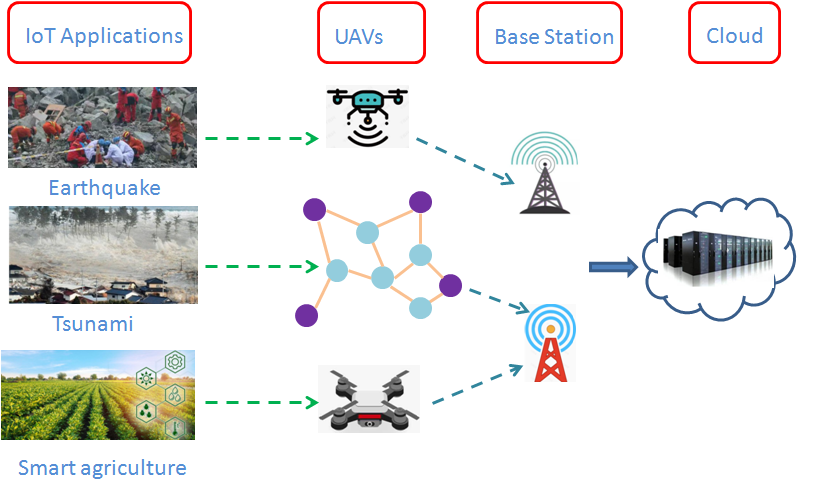
\includegraphics[width=4.2in,height=2.5in]{PPng.png} 
%\caption*{{\bf Fig.~4.}Divisible coin} \label{fig}

 \centering
\fontsize{6.5}{8}\selectfont {\small{\textbf{Fig. 1}. Network structure of edge computing with Multi-UAVs.}}
\end{figure}


%The main notations of this paper is illustrated in Table 1.



\begin{table}[H] %开始一个表格environment,表格的位置是h,here。
% \footnotesize
\caption{List of  main notations.} \label{tab2} %显示表格的标题
\setlength{\tabcolsep}{3.5mm}{
\scalebox{.9}[0.9]{
\begin{tabular}{cl} %设置了每一列的宽度,强制转换。

\toprule
\textbf{Symbol} & \textbf{Meaning}  \\ %用&来分隔单元格的内容 \\表示进入下一行


\midrule
 %画一个横线,下面的就都是一样了,这里一共有4行内容
$T$ & running time of the edge computing system\\

$t_h$ & time slot, $h\in Z^+$\\

$U$ & the group of users\\

$u_m$ & the $m$th user, $m\in Z^+$ \\

$S$ & the group of UAV edge nodes \\

$s_n$ & the $n$th UAV edge nodes, $m\in Z^+$\\

$C_s$ & the maximum data processing power of edge cloud\\

$d(s_1,s_2)$ & The internet transforming latency between  edge node $s_1$ and node $s_2$  \\
$x_{u,s,t}$ & the amount of tasks that user $u$ offloads to edge node $s$ at time slot $t$ \\
$\lambda_u$ & the total number of tasks\\
$q_{s,t}$ & the data processing capability of $s$ at time slot $t$\\
$E_O$ & operating cost of the edge computing system for all tasks\\
$E_Q$ & service quality cost of the edge computing system\\
$E_M$ & operating cost of the edge computing system for all tasks\\
$T_w(u,s)$ &  the waiting time for task $x_{u,s,t}$ in the transmission queue from user $u$ to edge node $s$ \\


\bottomrule
\end{tabular}}}
\end{table}


\subsection{Cost model}
The cost of the system is divided into three types: operation cost, QoS cost, and migration cost \cite{WANG}. Among them, the first two are static costs and are generated independently at each time slot. The migration cost is a dynamic cost, which depends on the task transfer decision during the task execution.


Operating cost: This cost mainly includes employing and  maintaining software, hardware resources,  CPU and storage costs, electricity costs, and carbon emissions costs. The maintenance cost is proportional to the number of tasks handled by each edge cloud. Operation unit cost represents the unit cost of edge node $s$ processing unit task quantity at time slot $t$, which is denoted by $a_{s,t}$. The operating cost of the edge computing system for all tasks is shown as formula(1):
\begin{equation}
E_O=\sum_{t\in T}\sum_{s\in S}a_{s,t}\sum_{u\in U}x_{u,s,t}        
\end{equation}

QoS cost: This cost is mainly used to represent the user quality of service. It is proportional to the network delay after users submit a service request to the system to process some task and return the associated result. It is assumed that all nodes in the system employ orthogonal frequency division multiple access (OFDMA) technology to communicate with other nodes. Transmission rules follows the first-in, first-out (FIFO) principle during transmission. Based on the M/G/1 queuing theory, the waiting time of task $x_{u,s,t}$ in the transmission queue from user $u$ to edge node $s$ is  calculated as follows \cite{WangX2020,Thomas2020}:

\begin{equation*}
T_w(u,s)=(\rho_{u,s,t}\overline{d}(u,s)+\rho_{u,s,t}\delta^2)/2(1-\rho_{u,s,t}\overline{d}(u,s)),      
\end{equation*}

 where $\overline{d}(u,s)$ is the average time delay for a task to transmit from $u$ to $s$; $\delta^2$ represents the variance of transmission delay; $\rho_{u,s,t}$ means transmission density. Denoted by $T_w=T_w(u,s)$, then, the total service quality cost of the edge computing system can be expressed as:
\begin{equation}
E_Q=\sum_{t\in T}\sum_{u\in U}(d(l_{u,t},s_{u,t}^{*})+T_w+\sum_{s \in S}\frac{x_{u,s,t}}{\lambda_u}\frac{q_{s,t}}{C_s}d(s_{u,t}^{*},s))     
\end{equation}

Migration cost: To optimize the cost, tasks often need to be migrated from one edge node to other edge nodes during task execution. Migration cost includes network bandwidth cost and migration delay cost. It is noted that the difference between the tasks in the two time slots is not equal to the migrated tasks. Because the edge cloud is constantly processing tasks at each time slot, the number of tasks completed at a time slot should be added to the difference between the two time slots to equal the amount of migrated tasks. We denoted the unit price of migrating unit task quantity by $b_s$. If function $(x)^{+}=\max\{x,0\}$ is defined, the total migration cost is calculated as follows:

\begin{equation}
E_M=\sum_{t\in T}\sum_{s\in S}b_s(\sum_{u\in U}x_{u,s,t}+q_{s,t-1}-\sum_{u\in U}x_{u,s,t-1})^{+}    
\end{equation}


Here, $(\sum_{u\in U}x_{u,s,t}+q_{s,t-1}-\sum_{u\in U}x_{u,s,t-1})^{+}$ represents the amount of tasks transferred by edge node $s$ in the process of transferring from time slot $t-1$ to time slot $t$. To simplify the expression, $\sum_{u\in U}x_{u,s,t}$ is denoted as $x_{s,t}$, that is, the sum of tasks assigned to edge cloud $s$ by all users at time slot $t$. Although task migration itself is dynamic and complex, the migration cost of an edge node is always directly related to the change of task volume. However, the migration amount is not equal to the difference between the tasks in the current time slot minus the tasks in the previous time slot. An example of task migration is shown in Fig 2. The blue circle indicates the effective radio signal coverage of $s_4$, and the green circle indicates the radio coverage of $s_3$. In  figure 2, both the signals of edge node $s_3$ and $s_4$ can cover user $u_1$, who is closer to $s_4$. The signal of $s_4$ will be stronger than that of $s_3$. Therefore, $u_1$ takes $s_4$ as the preferred node for network service. 


\begin{figure}[H]
\centering
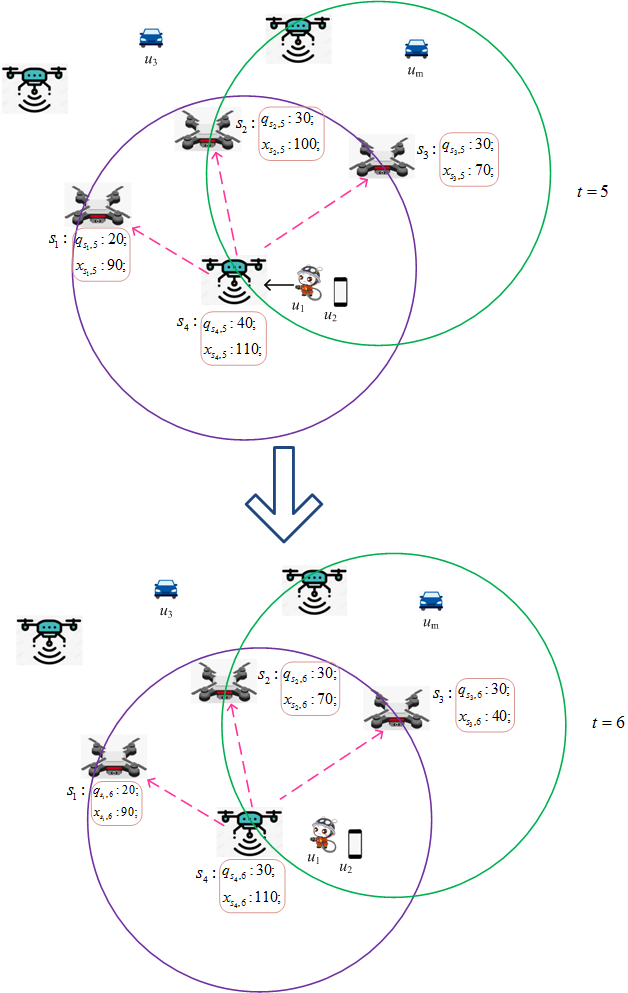
\includegraphics[width=3.8in,height=5.5in]{fig31.png} 
%\caption*{{\bf Fig.~4.}Divisible coin} \label{fig}

 \centering
\fontsize{6.5}{8}\selectfont {\small{\textbf{Fig.2}.  Task migration from time slot 5 to 6}}
\end{figure}
The total tasks of $s_1$ in the current slot 6 and the previous slot 5 are set to be 90, respectively. That is,  $x_{s_1,6}=x_{s_1,5}=90$, then, the task being migrited into edge node $s_1$  from time slot 5 to 6 can not be calculated by $x_{s_1,6}-x_{s_1,5}=90-90=0$ since the edge node $s_1$ is working all the time. Assuming $q_{s_1,5}=20$, then the task being migrated into $s_1$  from time slot 5 to 6 can be calculated as $90+20-90=20$. The calculation process of task migration  associated with Fig 2 is shown in Table 2. In actual operation, in order to reduce operation and maintenance costs and facilitate management, service providers may prefer to keep UAVs with the same model, which equipped with the same mission loads. Due to the change of working state, the available resources and real-time performance of the same UAV will also shift randomly. Therefore, it is reasonable and necessary to set different values of $q_{s,t}$ for UAVs in our experiment.

\begin{table}[h] %开始一个表格environment,表格的位置是h,here。
 \footnotesize
\caption{The calculation process of task migration  associated with Fig 2} %显示表格的标题
\begin{tabular}{c |c| c| c| c| c} %设置了每一列的宽度,强制转换。
\hline
Edge node  & \multicolumn{2}{|c|}{time slot 5} & \multicolumn{2}{|c|}{time slot 6} &  tasks moving into edge node\\  \cline{2-6} %用&来分隔单元格的内容 \\表示进入下一行
& $q_{s,5}$ & $x_{s,5}$  & $q_{s,6} $ & $x_{s,6}$ &  $(x_{s,t}+q_{s,t-1}-x_{s,t-1})^{+}$\\ \cline{2-6}
\hline %
$s_1$ & 20 & 90 & 20 & 90 & 20 \\
$s_2$ & 30 & 100 & 30  & 70 & 0 \\
$s_3$ & 30 & 70 & 30 & 40 & 0 \\
$s_4$ & 40 & 110 & 30 & 110 & 40\\
\hline
\end{tabular}
\end{table}



\subsection{Problem formulation}
The total cost of edge calculation can be expressed as the weighted sum of the three costs mentioned above, which can be expressed as:

\begin{equation}
P=E_O+E_Q+E_M
\end{equation}

The overall cost structure is illustrated in Fig. 3. We believe that these cost models are general enough and can capture a wide range of practical performance measures in an multi-UAVs enabled edge computing system from the perspective of edge cloud users.  Different from the stucture of \cite{WANG}, our cost function does not include reconstruction cost. Note that during the working process of an UAV, its software and hardware devices are always in a hot state. Thus, the hardware and software preparation time can be ignored. 

\begin{figure}[H]
\centering
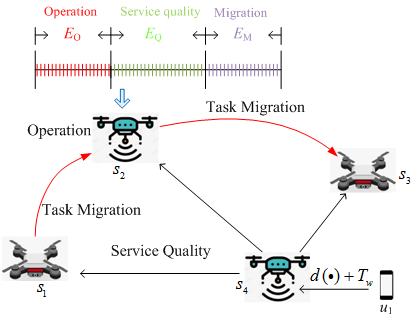
\includegraphics[width=2.8in,height=2.6in]{fig312.png} 
%\caption*{{\bf Fig.~4.}Divisible coin} \label{fig}

 \centering
\fontsize{6.5}{8}\selectfont {\small{\textbf{Fig.3}.  The overall cost structure of our multi-UAVs enabled edge computing system }}
\end{figure}


Without loss of generality, we have omitted the weighting coefficient in the above equation for simplicity, since the weighting coefficient can be implied in the parameters of each cost model, such as $a_{s,t}$ and $b_s$ in the expression form of Equation (4).  To solve the optimization problem of the total cost, the following linear programming problem is generated:
\begin{align}
\min P_0(t)=E_O+E_Q+E_M  \label{YY}\\
s.t.\quad
\sum_ux_{u,s,t} \le C_s, \forall s,\forall t  \tag{\ref{YY}{a}} \label{YYa}\\
\sum_sx_{u,s,t} \ge \lambda_u, \forall u,\forall t \tag{\ref{YY}{b}} \label{YYb}\\
\sum_ukx_{u,s,t} \le Q_s, \forall u,\forall t \tag{\ref{YY}{c}} \label{YYc}\\
 x_{u,s,t} \ge 0, \forall u, \forall s ,\forall t \tag{\ref{YY}{d}} \label{YYd}
\end{align}


Constraint condition (5a) ensures that the sum of all tasks assigned to the edge cloud does not exceed its computing and storage capacity. Constraint condition (5b) ensures that all tasks are assigned, and greater-than character ensures that the system remains redundant.  $k$ represents the power consumption coefficient of unit task quantity, and the constraint condition (5c) ensures that the sum of all tasks assigned to the edge cloud $s$ will not exceed the battery limit of UAVs. Let $Z_s=min\{Q_S /k,C_s\}$, then constraint conditions (5a) and (5c) are combined into:

\begin{align}
\sum_u x_{u,s,t}\le Z_s, \forall s ,\forall t  \tag{\ref{YY}{e}} \label{YYe}
\end{align}
%%%%%%%%%%%%%%%%%%%%%%%%%%%%%%%%%%%%%%%%%%
\section{Online Algorithm Design}
Since each edge node cannot obtain the state information of the whole system in a distributed environment, we introduce a competitive ratio to estimate the efficiency of the proposed online algorithm solution. The competitive ratio is the optimization results of an online algorithm with limited information to an offline algorithm with all information.
\subsection{Algorithm design}
Next, we will solve the above problems based on regularization technique \cite{ZHANG K Y,WANG}. The pseudo code of our proposed PSEC is listed in Table 3. At each time slot $t$, taking the user's current position $l_{u,t}$ and the task $x_{u,s,t-1}$ assigned at the previous time slot $t-1$ as input, the optimization problem $P_1(t)$ in the current time slot $t$ can be obtained:

\begin{table}[h] %开始一个表格environment,表格的位置是h,here。
 \footnotesize
\caption{The pseudo code of our proposed PSEC} %显示表格的标题
\begin{tabular}{p{8cm}} %设置了每一列的宽度,强制转换。

\hline
\textbf{Algorithm 1}  \\ %用&来分隔单元格的内容 \\表示进入下一行


\hline %画一个横线,下面的就都是一样了,这里一共有4行内容
1:caculate original total cost $P_0$\\
2:regularize the objective $P_0$ to $P_1$\\
3:$P_1$ is transformed into linear programming problem $P_2$\\
4:initialize parameters \\
5:for $u \in U$\\
6:\quad for $s\in S$\\
7:\quad \quad for $t\in T$\\
8:\quad \quad update $P_2$ according to fomula(8)\\
9:\quad \quad solve $P_2$ via convex programming\\
10:\quad \quad $t=t+1$\\
11:\quad \quad end for\\
12: \quad end for\\
13: end for\\
\hline
\end{tabular}
\end{table}



 \begin{equation}
\begin{aligned}
\min P_1(t)&=\sum_{s\in S}a_{s,t}\sum_{u\in U}x_{u,s,t}+\\
&\sum_{u\in U}(d(l_{u,t},s_{u,t}^{*})+T_w+\sum_{s\in S}\frac{x_{u,s,t}}{\lambda_u}\frac{q_{s,t}}{C_s}d(s_{u,t}^{*},s))+\\
&\sum_{s\in S}\frac{b_s}{\eta_s}((x_{s,t}+q_{s,t-1}+\varepsilon)\ln \frac{x_{s,t}+q_{s,t-1}+\varepsilon }{x_{s,t-1}^{*}+\varepsilon }-x_{s,t}-q_{s,t-1})\label{LL} 
\end{aligned}
 \end{equation}
 s.t.
 \begin{align}
\sum_s x_{u,s,t} \ge \lambda_u, \forall u  \tag{\ref{LL}{a}} \label{LLa}\\
\sum_{f\in S \backslash s} x_{u,f,t} \ge \sum_{u\in U}\lambda_u-Z_s, \forall s \tag{\ref{LL}{b}}\\ x_{u,s,t} \ge 0, \forall u, \forall s \tag{\ref{LL}{c}} \label{LLc}
\end{align}

Here, both  $\eta_s=\ln(1+Z_s/\varepsilon)$ and $\varepsilon$ are parameters which are greater than 1. Obviously, the objective function $P_1(t)$ is a convex function with linear constraints, thus we can use any convex programming solution to search the solution of $P_1(t)$. By combining the optimization solution $x_{u,s,t}^{*}$ obtained by $P_1(t)$ at each time slot $t$, the approximate optimization solution $\{x_{u,s,t}^{*}|0\le t \le t_h\}$ of the original problem $P_0(t)$ is obtained, which is the task allocation strategy of edge computing. Next, we prove that the optimization solution $\{x_{u,s,t}^{*}|0\le t \le t_h\}$ is the solution of the optimization problem $P_0(t)$.


\textbf{Theorem 1}(Validity). The optimal solution $\{x_{u,s,t}^{*}|0\le t \le t_h\}$ of $P_1(t)$ at each time slot constitutes a solution of $P_0(t)$.


Proof: It is proved that the optimal solution of $P_1(t)$ also satisfies the constraints (5b), (5d) and (5e) in $P_0(t)$. Since $x_{u,s,t}^{*}$ is the optimal solution of $P_1(t)$ at time slot $t$, $\forall t,x_{u,s,t}^{*}$ makes (6a) and (6c) valid, thus (5b) and (5d) are valid. Next,  we prove constraint (5e) is also true:


Because

\begin{equation*}
\frac{\partial P_1(t)}{\partial x_{u,s,t}}=a_{s,t}+\frac{q_{s,t}}{\lambda_u C_s}d(s_{u,t}^{*},s)+\frac{b_s}{\eta_s}\ln\frac{x_{s,t}+q_{s,t-1}+\varepsilon}{x_{s,t-1}^{*}+\varepsilon-1}+\frac{b_s}{\eta_s}(x_{s,t-1}^{*}+q_{s,t-1}+\varepsilon)>0,
\end{equation*}


from the above equation, we can obtain that $\forall u, \forall s, \forall t$, the function $P_1(t)$ is monotonically increasing on the interval $[x_{u,s,t}^{*},+\infty)$ with respect to $x_{u,s,t}$. Without losing generality, let's assume $x_{u,s,0}=0$ and $x_{s,0}^{*}=\sum_{u\in U}x_{u,s,t}^{*}=0$. The following is a proof by mathematical induction. When $ t=1$, and $x_{u,s,1}$ represents an optimal solution of $P_1(t)$. Then, there must be $x_{s,1}^{*}=\sum_{u\in U}x_{u,s,1}^{*}\le Z_s$. Otherwise, if $ x_{u,s,1}^{*}\ge Z_s $ or $ x_{s,1}^{*}\ge Z_s $,   then, $ x_{u,s,1}^{`}= Z_s $ and $ x_{s,1}^{`}= Z_s $ is a new optimal solution for the problem $P_1(t)$ . Obviously, this new optimal solution leads to a smaller target value for $P_1(t)$, which contradicts the hypothesis. Similarly, the same conclusion can be reached when $0\le t \le t_h$.

\subsection{Complex analysis}

At each time slot, the solution of $P_1(t)$ can be obtained by solving the convex programming problem. Therefore, the algorithm proposed by us is solvable in polynomial time \cite{Bubeck2015}. Here, we can choose the interior point algorithm to solve our problem, then the time complexity of our algorithm is $O((mn))^{3.5}$, where $mn$ is the number of variables in function $P_1(t)$, $m$ is the number of edge nodes, and $n$ is the number of users.
\section{Competition Analysis}

The efficiency analysis of the proposed scheme is given through competition analysis. Competition analysis mainly uses competitive ratio to analyze the efficiency of online algorithms. The method is to compare the efficiency of an online algorithm with that of an offline algorithm where all input conditions are known in advance. The basic steps of the analysis are as follows:
\begin{itemize}

    \item The relaxation of programming problem $P_0(t)$ is transformed into linear programming problem $P_2(t)$ by auxiliary variables $y_{s,t}$ and $z_{s,t}$.

    \item Derive the duality problem $D$ of $P_2(t)$.

    \item Construct an efficient solution of problem $D$ by a solution of $P_1(t)$.
\end{itemize}


  Our goal is to derive the inequality \cite{WANG} :
\begin{equation}
P_0(t)\ge P_2(t) \ge D \ge \frac{1}{r} P_1(t)
\end{equation}


Since $ P_2(t)$ is a relaxation of the constraint on $ P_0(t)$, $ P_0(t) \ge P_2(t)$ is true. We know $ P_2(t) \ge D$ from the weak duality theorem. The last inequality is deduced by comparing the solutions of $D$ and $ P_1(t)$.  The existence of all the above inequalities guarantees that the proposed algorithm is $r$ competition, where the competitive ratio $r$ will be given later in Lemma 4. The specific analysis process is shown below.
\subsection {Auxiliary planning problem}
By introducing auxiliary variables $y_{s,t}$ and $z_{s,t}$, the nonlinear programming problem $P_0(t)$ is reconstructed to obtain the relaxed linear programming problem $P_2(t)$. We also give the lower bound of the relaxation variable, and the formula of $P_2(t)$ is shown as follow:
\begin{align}
&\min P_2(t)=\sum_{s\in S}\sum_{t\in T}\sum_{u\in U}a_{s,t}x_{u,s,t}+\sum_{s\in S}\sum_{t\in T}\sum_{u\in U}\frac{x_{s,u,t}}{\lambda_u}\frac{q_{s,t}}{C_s} +\sum_{s\in S}\sum_{t\in T}b_s y_{s,t} \label{BB}\\
s.t.\quad
&y_{s,t}\ge\sum_{u\in U}x_{u,s,t}+q_{s,t-1}-\sum_{u\in U}x_{u,s,t-1}, \forall s, \forall t  \tag{\ref{BB}{a}} \label{BBa}\\
&\sum_{f\in S\backslash s}x_{u,f,t}\ge (\sum_{u\in U}\lambda_{u}-Z_s)^{+},\forall s,\forall t \tag{\ref{BB}{b}} \label{BBb}\\
&y_{s,t}\ge 0, \forall s, \forall t \tag{\ref{BB}{c}} \label{BBc}\\
&(5b),(5d) \tag{\ref{BB}{d}} \label{BBd}
\end{align}

When the connection between the user and the base station is established and the user queuing model is determined, $\sum_{t \in T}\sum_{u\in U}(d(l_{u,t},s_{u,t}^*)+T_w)$ is independent of task allocation strategy, thus this part of cost is not considered in Equation (8).

 Next, we give the Lagrangian dual $D$ of $P_2$. Let $\alpha_{s,t},\rho_{s,t}$ ,and $\theta_{u,t}$ be dual variables of equations (8a), (8b) and (5b) respectively. Let $h_{u,s}$ be the indicator variable associated with a user and edge cloud, namely, if user $u$ has tasks assigned to $s$, $h_{u,s}=1$; otherwise, $h_{u,s} =0$. Duality programming problem $D$ is as follows:

\begin{align}
&\max D=\sum_{t\in T}\sum_{u\in U}\lambda_u h_{u,s}\theta_{u,t}+\sum_{t\in T}\sum_{s\in S}(\sum_{u\in U} \lambda_u-Z_s)^{+}\rho_{s,t}  \label{JJ}\\
s.t. \quad
&-a_{s,t}-g_{s,u}\frac{q_{s,t}}{\lambda_u C_s}d(s_{u,t}^{*},s)+\alpha_{s,t+1}-\alpha_{s,t}+\sum_{f\in S \backslash s}\rho_{f,t}+g_{s,u}\theta_{u,t}\le 0 ,\forall u, \forall s, \forall t \tag{\ref{JJ}{a}} \label{JJa}\\
&-b_s+\alpha_{s,t}\le 0 , \forall s, \forall t \tag{\ref{JJ}{b}} \label{JJb}\\
&\alpha_{s,t}\ge 0 , \rho_{s,t}\ge 0 ,\forall s, \forall t  \tag{\ref{JJ}{c}} \label{JJc}\\
&\theta_{u,t}\ge 0,\forall u, \forall t \tag{\ref{JJ}{d}} \label{JJd}
\end{align}


At the same time, we can obtain the Karush-Kuhn-Tucker (KKT) condition of $P_1(t)$. Let the dual variables related to constraints (6a),(6b) and (6c) be $\theta_{u,t}^{`}$, $\rho_{f,t}^{`}$ and $\delta_{u,s,t}^{`}$,  respectively. The following formula we could obtain:
%\begin{equation}
\begin{align}
&a_{s,t}+g_{s,u}\frac{q_{s,t}}{\lambda_u C_s}d(s_{u,t}^{*},s)+\frac{b_s}{\eta_u}\ln \frac{x_{s,t}+q_{s,t-1}+\varepsilon}{x_{s,t-1}^{*}+\varepsilon}-g_{s,u}\theta_{u,t}^{`}-\sum_{f\in S \backslash s} \rho_{f,t}^{`}-\delta_{f,t}^{`}=0, \forall s, \forall u  \label{SS}\\
s.t.\quad
&\theta_{u,t}^{`}(\lambda_u-\sum_{s}x_{u,s,t})=0, \forall u \tag{\ref{SS}{a}} \label{SSa}\\
&\rho_{f,t}^{`}(\sum_{u\in U}\lambda_u-Z_s-\sum_{f\in S \backslash s}x_{u,f,t})=0, \forall s \tag{\ref{SS}{b}} \label{SSb}\\
&\delta_{u,s,t}^{`}x_{u,s,t}=0, \forall u ,\forall s \tag{\ref{SS}{c}} \label{SSc}\\
&(6a)(6b)(6c), \theta_{u,t}^{`}\ge 0, \rho_{f,t}^{`}\ge 0 \forall s , \forall u  \tag{\ref{SS}{d}} \label{SSd}
\end{align}
%\end{equation}

Where (10) is based on stability, and  (10b), (10c), and (10d) are based on complementary relaxation conditions. Using an optimal solution $x_{u,s,t}^{*}$ of $P_2(t)$ and dual variables $\theta_{u,t}^{`}$ and $\rho_{u,t}^{`}$,  an optimal solution $S_D$ of the dual programming problem $D$ can be constructed through  following formulas:

\begin{align*}
\alpha_{s,t}&=\frac{b_s}{\eta_s}\ln \frac{C_s+\varepsilon}{x_{s,t-1}^{*}+\varepsilon}\ge 0 ,\\
\theta_{u,t}&=\theta_{u,t}^{`},\\
\rho_{u,t}&=\rho_{u,t}^{`}.
\end{align*}

\textbf{Lemma 1}. $S_D$ is a valid solution of the programming problem $D$.


Proof:
We first derive some preliminaries. For $\alpha_{s,t}$ we have\\
\begin{align*}
&-(\alpha_{s,t+1}-\alpha_{s,t})\\
=&\frac{b_s}{\eta_s}\ln \frac{C_s+\varepsilon}{x_{s,t-1}^{*}+\varepsilon}-\frac{b_s}{\eta_s}\ln \frac{C_s+\varepsilon}{x_{s,t}^{*}+\varepsilon}\\
=&\frac{b_s}{\eta_s}\ln \frac{x_{s,t}^{*}+\varepsilon}{x_{s,t-1}^{*}+\varepsilon}\\
\end{align*}
Based on the above equation, we have\\
\begin{align*}
&-a_{s,t}-g_{s,u}\frac{q_{s,t}}{\lambda_u C_s}d(s_{u,t}^{*},s)+\alpha_{s,t+1}-\alpha_{s,t}+\sum_{f \in S\backslash s } \rho_{f,t}+g_{s,u}\theta_{u,t}\\
=&-a_{s,t}-g_{s,u}\frac{q_{s,t}}{\lambda_u C_s}d(s_{u,t}^{*},s)-\frac{b_s}{\eta_s}\ln \frac{x_{s,t}^{*}+\varepsilon}{x_{s,t-1}^{*}+\varepsilon}+\sum_{f\in S \backslash s}\rho_{f,t}+g_{s,u}\theta_{u,t}\le 0,\\
\end{align*}
where the inequality in the last line follows from equation $(10)$. The above inequality indicates that the constraint $(9a)$  is satisfied by the solution $S_D$. Constraint $(9b)$ is satisfied by the following inequality. 
\begin{align*}
\alpha_{s,t}=&\frac{b_s}{\eta_s}\ln \frac{C_s+\varepsilon}{x_{s,t-1}^{*}+\varepsilon}\\
=&\frac{b_s}{\ln (1+C_s / \varepsilon)}(\ln (1+C_s / \varepsilon)- \ln (1+x_{s,t-1}^{*} / \varepsilon))\\
=&b_s(1-\frac{\ln(1+x_{u,s,t}^{*}/ \varepsilon)}{\ln(1+C_s/ \varepsilon)})\le b_s.
\end{align*}

That is to say, (9a)  and (9b) are true.  According to the definition and the construction of the optimal solution, (9c) and (9d) are established.  Therefore, the solution $S_D$ of $D$ constructed based on the solution of $P_2(t)$ satisfies all constraints of $D$. $\square$ 


\subsection{Competitive ratio}

Next, we will analyze the competitive ratio $r$.  First we divide $P_1(t)$ into two parts, the static cost part $E_O+E_Q$ and the dynamic cost part $E_M$, and then prove that each part is bounded. Then we combine the two parts to prove that the population is bounded and deduce the competitive ratio $r=1+\gamma n_0 $, where $\gamma$ and $n_0$ will be defined later in Lemma 4.  


\textbf{Lemma 2}. $D$ is the upper bound of operation cost and QoS cost in problem $P_0(t)$. 

 
We first show the proof of the following preliminary results that will be used in the proof of lemma 2.

\textbf{Lemma 3}. $\forall s, \sum_{t\in T}x_{s,t}^{*}\ln \frac{x_{s,t}^{*}+q_{s,t-1}+\varepsilon}{x_{s,t-1}^{*}+\varepsilon} \ge 0 $.


Proof. We separate the $\sum_{t\in T}x_{s,t}^{*}\ln \frac{x_{s,t}^{*}+\varepsilon}{x_{s,t-1}^{*}+\varepsilon}$ into two parts $\sum_{t\in T}(x_{s,t}^{*}+\varepsilon)\ln \frac{x_{s,t}^{*}+\varepsilon}{x_{s,t-1}^{*}+\varepsilon}$ and $\sum_{t\in T}\varepsilon\ln \frac{x_{s,t-1}^{*}+\varepsilon}{x_{s,t}^{*}+\varepsilon}$. Then, we deduce the two lower bounds of both parts one by one, the two bounds together will form a lower bound for the added formula. The detailed  proof process is as follows.

\begin{align*}
&\sum_{t\in T}x_{s,t}^{*}\ln\frac{x_{s,t}^{*}+q_{s,t-1}+\varepsilon}{x_{s,t-1}^{*}+\varepsilon} \\
\ge & \sum_{t\in T}x_{s,t}^{*}\ln \frac{x_{s,t}^{*}+\varepsilon}{x_{s,t-1}^{*}+\varepsilon}\\
=&\sum_{t\in T}(x_{s,t}^{*}+\varepsilon)\ln \frac{x_{s,t}^{*}+\varepsilon}{x_{s,t-1}^{*}+\varepsilon}+\sum_{t\in T}\varepsilon\ln \frac{x_{s,t-1}^{*}+\varepsilon}{x_{s,t}^{*}+\varepsilon}\\
\ge & ( \sum_{t\in T}(x_{s,t}^{*}+\varepsilon))\ln \frac{ \sum_{t\in T} x_{s,t}^{*}+\varepsilon }{ \sum_{t\in T} x_{s,t-1}^{*}+\varepsilon } +\sum_{t\in T}\varepsilon\ln \frac{x_{s,t-1}^{*}+\varepsilon}{x_{s,t}^{*}+\varepsilon}\\
\ge & \sum_{t\in T}(x_{s,t}^{*}+\varepsilon)- \sum_{t\in T}(x_{s,t-1}^{*}+\varepsilon)+ \sum_{t\in T}\varepsilon (\ln(x_{s,t-1}^{*}+\varepsilon)- \ln(x_{s,t}^{*}+\varepsilon)) \\
=&(x_{s,t_h}^{*}+\varepsilon)- (x_{s,t_0}^{*}+\varepsilon)+\varepsilon \ln((x_{s,t_0}^{*}+\varepsilon)/( x_{s,t_h}^{*}+\varepsilon))\\
=& x_{s,t_h}^{*}+\varepsilon \ln(\varepsilon/( x_{s,t_h}^{*}+\varepsilon))\\
\ge & x_{s,t_h}^{*}+\varepsilon-(x_{s,t_h}^{*}+\varepsilon)=0,
\end{align*}

The second inequality above holds based on the following inequality:


$\sum_i p_i \ln p_i /q_i \ge \sum_i p_i \ln \sum_i p_i/ \sum_i q_i, \forall p_i >0,\forall q_i>0,$


The third inequality above holds based on the following inequality:


$p \ln p /q \ge p-q, \forall p >0,q>0$.$\square$


Then, we can obtain the upper bound of $E_O+E_Q$ and give the detailed proof of Lemma 2 as follows:

Proof.  The derivation is conducted by applying the equations $(10)-(10d)$ obtained from the Karush-Kuhn-Tucker (KKT) condition $P(1)$.  Note that $\sum_{t \in T}\sum_{u\in U}(d(l_{u,t},s_{u,t}^*)+T_w)$ is omitted as in objective $P_2(t)$. 

\begin{align*}
&\sum_{t\in T}\sum_{s\in S}a_{s,t}\sum_{u\in U}x_{u,s,t}+\sum_{t\in T}\sum_{s\in S} \sum_{u\in U}\frac{x_{u,s,t}}{\lambda_u}\frac{q_{s,t}}{C_s}d(s_{u,t}^{*},s)\\
=&\sum_{t\in T}\sum_{s\in S} \sum_{u\in U} x_{u,s,t}(-\frac{b_s}{\eta_u}\ln \frac{x_{s,t}+q_{s,t-1}+\varepsilon}{x_{s,t-1}^{*}+\varepsilon}+g_{s,u}\theta_{u,t}^{`}+\sum_{f\in S \backslash s}\rho_{f,t}^{`}+\delta_{u,s,t}^{`})\\
\le & \sum_{t\in T}\sum_{s\in S} \sum_{u\in U} x_{u,s,t}( g_{s,u}\theta_{u,t}+\sum_{f\in S\backslash s}\rho_{f,t}+\delta_{u,s,t})\\
= & \sum_{t\in T}\sum_{u\in U}\lambda_u g_{s,u}\theta_{u,t}+\sum_{t\in T}\sum_{s\in S}\rho_{s,t}(\sum_{u\in U}\lambda_u-Z_s) \\
\le & \sum_{t\in T}\sum_{u\in U}\lambda_u g_{s,u}\theta_{u,t}+\sum_{t\in T}\sum_{s\in S}\rho_{s,t}(\sum_{u\in U}\lambda_u-Z_s)^{+}=D.
\end{align*}
where the equation in the first line is obtained according to $(10)$,   the inequality in the second line is obtained by applying Lemma 2 and Lemma 3,  the equality in the third line follows by $(10a)-(10d)$. $\square$

\textbf{Lemma 4}. $\gamma n_0 D$ is an upper bound on migration cost in problem $P_0(t)$, where $\gamma=\max\{(Z_s+\varepsilon)\eta_s\}$, $n_0$ is the number of edge nodes.  


Proof.  For facilitate narration, set

 \quad $S_t^{+}= \{s|s\in S \cap (x_{s,t}^{*}+q_{s,t-1})>x_{s,t-1}^{*}\}$,

according to the definition $(x)^+=max\{x,0\}$, we have  


\begin{align*}
&\sum_{t\in T}\sum_{s\in S}b_s(\sum_{u\in U}x_{u,s,t}+q_{s,t-1}-\sum_{u\in U}x_{u,s,t-1})^{+}\\
= & \sum_{t\in T}\sum_{s\in S_t^{+}} b_s (x_{s,t}^{*}+q_{s,t-1}- x_{s,t-1}^{*}) \\
\le & max\{(Z_s+\varepsilon)\eta_s\}\sum_{t\in T}\sum_{s\in S_t^{+}} \frac{b_s}{\eta_s}\ln \frac{ x_{s,t}^{*}+q_{s,t-1}+\varepsilon }{ x_{s,t-1}^{*}+\varepsilon }\\
\le & \gamma \sum_{t\in T}\sum_{s\in S} \sum_{u\in U} (g_{s,u}\theta_{u,t}+\sum_{f\in S \backslash s}\rho_{f,t}) \\
\le & \gamma \sum_{t\in T}\sum_{s\in S} \sum_{u\in U} (g_{s,u}\theta_{u,t}+\sum_{f\in S \backslash s}\rho_{f,t})\lambda_u \\
\le & \gamma n_0(\sum_{t\in T} \sum_{u\in U}\lambda_u g_{s,u}\theta_{u,t}+\sum_{t\in T}\sum_{s\in S}\rho_{s,t}(\sum_{u\in U}\lambda_u-Z_s)^{+}) =\gamma n_0 D.
\end{align*}

where, $\lambda_u\ge 1$. The equation in the first line is obtained by applying the definition $(x)^+=max\{x,0\}$, the inequality in the second line follows by the $p-q\leq ln\frac{p}{q}$ for any $p>0,~q>0$. Therefore, the
proof is completed. $\square$

Combining all the results in Theorem 1, Lemma 3, and Lemma 4, the following theorem on the competitive ratio can be obtained for our proposed PSEC algorithm.


\textbf{Theorem 2}.  PSEC generates feasible solutions to $P_0$ with a competitive ratio $r=1+\gamma n_0$.

\section{Simulated Analysis}
In this section, the performance of the  PSEC algorithm is simulated in PC that has
disposition with the Intel Core I5-9300H processor, 8 GB RAM and 512GB solid drive. The simulation platform uses MATLAB 2020a. The simulation scene is set within $100m*100m$. The users and  edge nodes move randomly within the range.  The capacity $C_s$ of each edge node is set to be $[6000,8000,10000,12000,14000,16000]$Mb.  The essential parameters and
the scope of values are indicated in Table 4. Using the method of randomly generating workload, the distribution of task quantity satisfies the constraint condition (6a-6c), and the influence of different users and nodes on communication price is studied in the delay scenes. For further analysis, we compare our proposed PSEC algorithm with MOERA \cite{WANG} algorithm and MEH\cite{LiW21} algorithm, respectively. The MEH  is based on M/M/c queue to capture the execution process of tasks in MEC server with the optimal offloading probability $(p =0.35)$. Where, the task arrival rate is denoted by $\lambda=0.3$, and task service rate is denoted by $\mu=0.5$. 

\begin{table}[h] %开始一个表格environment,表格的位置是h,here。
 \footnotesize
\caption{Experiment parameters} %显示表格的标题
\begin{tabular}{p{2cm}p{6cm}} %设置了每一列的宽度,强制转换。

\hline
Parameters&Default values  \\ %用&来分隔单元格的内容 \\表示进入下一行



\hline %画一个横线,下面的就都是一样了,这里一共有4行内容
$T(s)$ &$3600$\\

$|U|$&$[5,10,15,20,25,30]$\\
$|S|$&$[5,10,15,20,25,30]$\\
$q_{s,t}(Mb)$&$[64,128,256,512,1024,2048]$\\
$C_s(Mb)$&$[6000,8000,10000,12000,14000,16000]$\\
$Qs/k$ & 100000\\
$\varepsilon$&$[0.001,0.01,0.1,1,10,100,1000]$\\
$a_{u,s,t}$&$\sim$ U(0,1)\quad ($a_{u,s,t}$ follows the  uniform distribution)\\
$b_s$&$\sim$ U(0,1)\quad ($b_s$ follows the  uniform distribution)\\
$\rho_{u,s,t}$&$\sim P(0.5)$\quad($\rho_{u,s,t}$ follows the  poisson distribution)\\
\hline
\end{tabular}
\end{table}

Fig.4 depicts the interrelationship between the operating cost, QoS cost and migration cost with different users.  The three costs $E_Q,E_M$ and $E_O$, are defined by the formulas (1), (2) and (3),  respectively. It is obvious that the QoS cost increases rapidly with the increase of the number of users. The reason is that the QoS cost is affected by the communication distance. For mobile edge computing, the user is moving all the time, and the distance from each user to the associated  edge node  will varies randomly, which will significantly affect the user's QoS cost. The $E_O$  hardly changes with the number of users since it only depends on the number of tasks processed in each time slot. When the number of users increases from 5 to 10, the migration cost $E_M$ increases rapidly.  However, when the number of users changes between 10 and 30, $E_M$  tends to be stable. This is because when the number of users is small, migrating tasks from busy nodes to idle nodes will significantly reduce the total time cost, and the migration volume is large. When the number of users is greater than 10, all edge nodes enter busy state, thus, the migration of tasks has little effect on the reduction of the total cost. 

 The performance affected by different  number of edge nodes is shown in   Fig.5.  When number of edge nodes becomes larger, the operation cost  increase lareger. This is because when a UAV is deployed to the edge network, even if it does not undertake any edge computing task, it still needs to consume  operation cost. The number of UAVs is not the more the better, it should be deployed according to actual needs. The migration cost does not increase with the increase of the number of edge nodes. This is mainly because as the task volume remains unchanged, too much migration may lead to the increase of the total cost. In terms of the $E_Q$, it decreases as the number of edge nodes increases.  It can be seen  that when the number of UAVs increases, the operation cost of UAVs will increase, but the QoS cost will decrease. Therefore, the number of UAVs is not the more the better, it should be determined according to the total cost requirements. 

\begin{figure}[H]
\centering
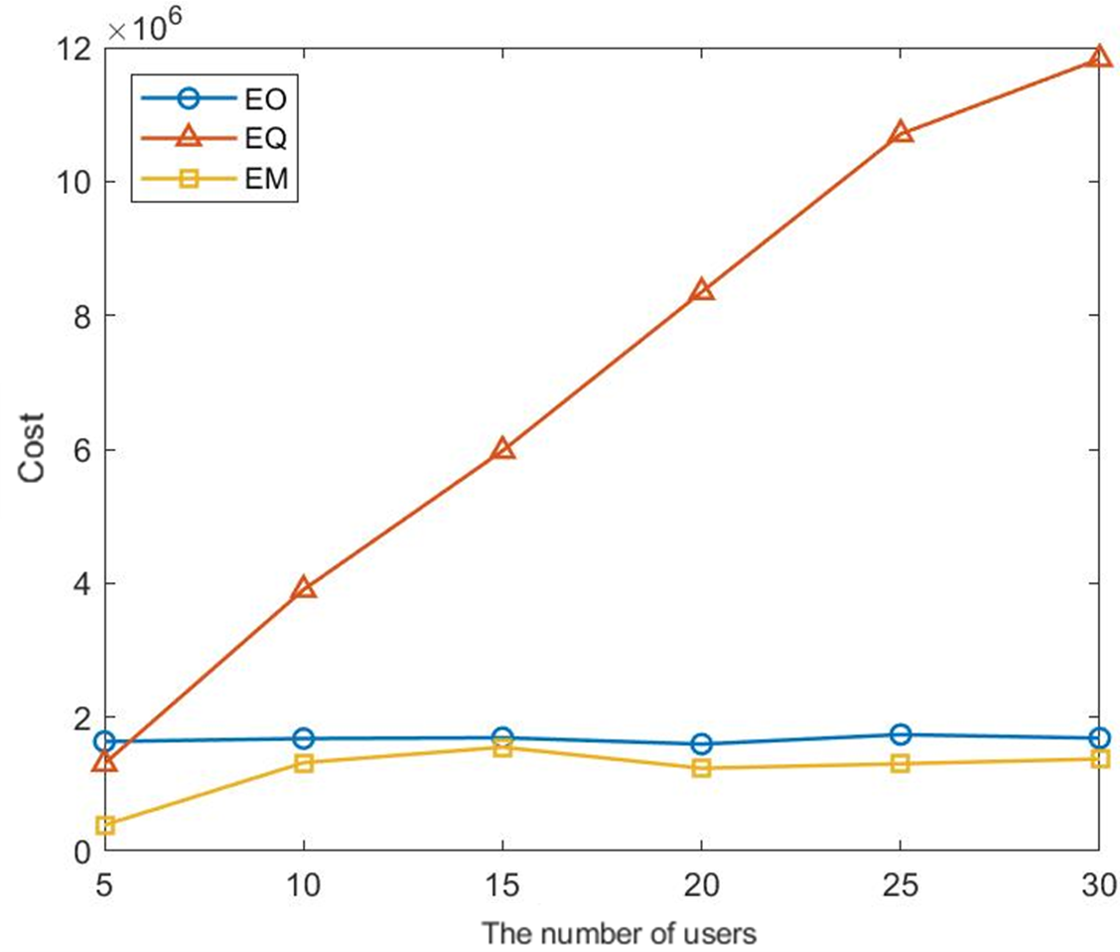
\includegraphics[width=3.2in,height=2.5in]{fig2a.png} 
%\caption*{{\bf Fig.~4.}Divisible coin} \label{fig}

 \centering
\fontsize{6.5}{8}\selectfont {\small{\textbf{Fig. 4}. Impact of different users’ number on three costs.}}
\end{figure}
\begin{figure}[H]
\centering
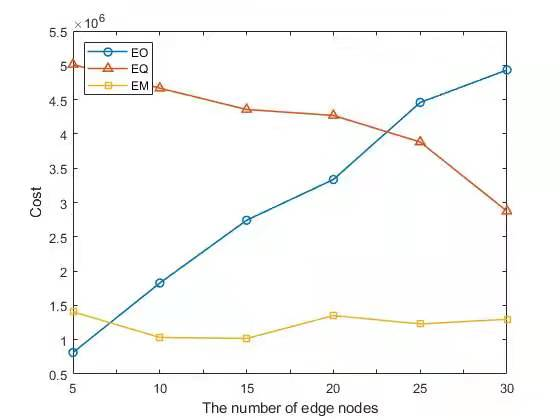
\includegraphics[width=3.5in,height=2.6in]{fig2b2.jpg} 
%\caption*{{\bf Fig.~4.}Divisible coin} \label{fig}

 \centering
\fontsize{6.5}{8}\selectfont {\small{\textbf{Fig. 5}. Impact of different edge nodes’ number on three costs.}}
\end{figure}
Fig. 6 illustrates the performance comparison with randomly moving edge nodes under various number of users.   When the number of users increases, the total costs of the three schemes are increasing, respectively. When the number of users is less than 10, the cost of our PSEC is slightly higher than that of the MEH. When the number of users is greater than 10, the cost of the MEH increases rapidly, and the cost growth of our consumption is not obvious. For different number of users, the cost of our PSEC always accounts for about half of the MOERA's cost.  From the perspective of the number of users, our proposed PSEC has achieved a more gentle growth. Futhermore, when the number of users is greater than 10, our PSEC  can save about $50\%$ of the total cost.

Fig. 7 shows that the  PSEC method can provide users with the lowest cost edge computing services under the different number of edge nodes. When the number of edge nodes is 5, the cost of the three methods is almost the same. But when the number of nodes increases, the cost of the three methods increases significantly to provide better service and faster response. However, the PESC method can always require the lowest total cost, which is at least  $20\%$ less  than the other two schemes. Through comprehensive comparison in Fig.6 and Fig.7,  the PSEC method is less sensitive to the number of users and nodes. Thus, our PSEC can be applied to complex scenes  and has strong robustness.
\begin{figure}[H]
\centering
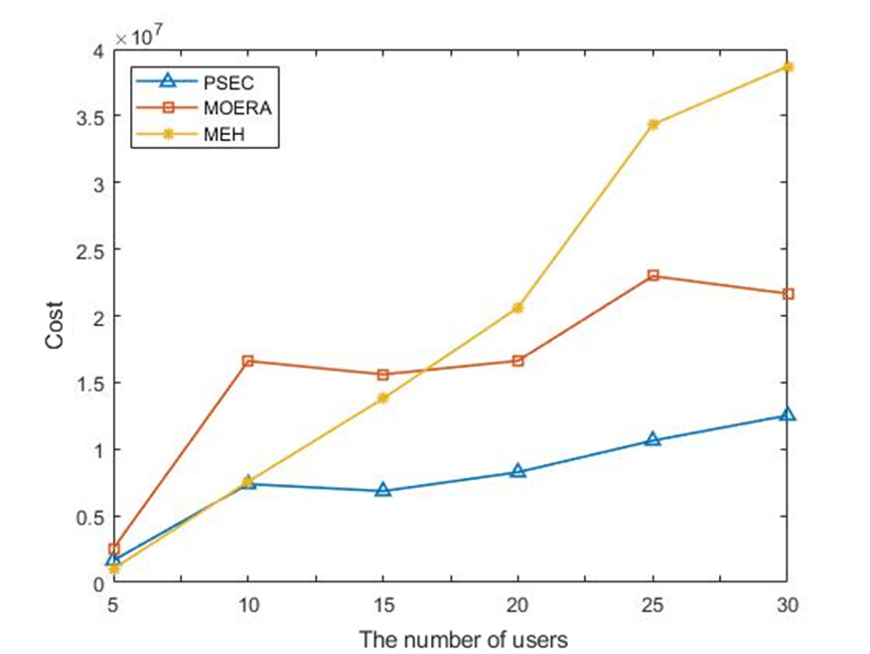
\includegraphics[width=3.2in,height=2.5in]{fig3a.png} 
%\caption*{{\bf Fig.~4.}Divisible coin} \label{fig}

 \centering
\fontsize{6.5}{8}\selectfont {\small{\textbf{Fig.6}.  Impact of number of users on total cost}}
\end{figure}
\begin{figure}[H]
\centering
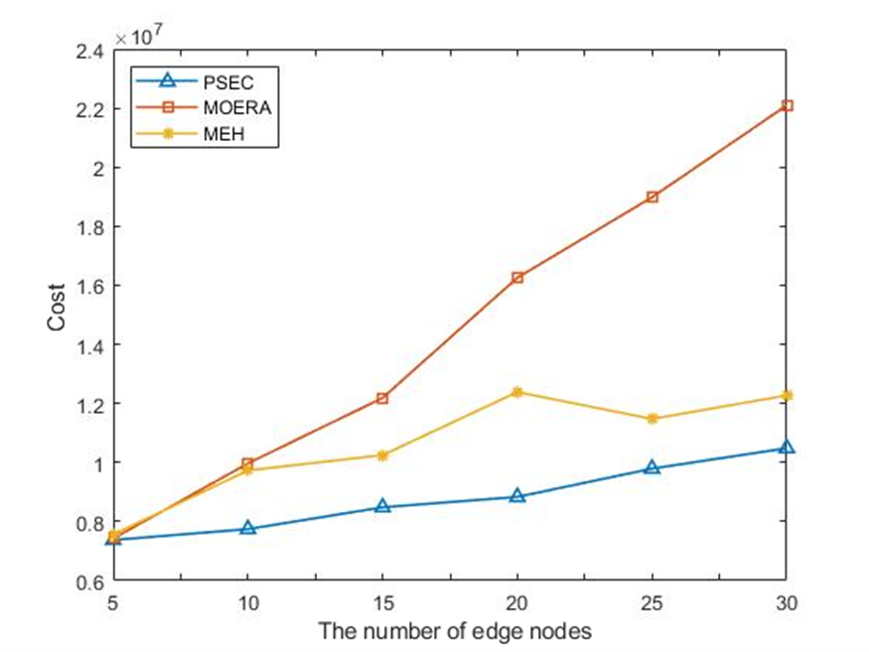
\includegraphics[width=3.2in,height=2.5in]{fig3b.png} 
%\caption*{{\bf Fig.~4.}Divisible coin} \label{fig}

 \centering
\fontsize{6.5}{8}\selectfont {\small{\textbf{Fig.7}.Impact of number of edge nodes on total cost}}
\end{figure}

In Fig.8, we reveal the relationship between the system performance and the  parameter factor $\varepsilon$. According to the parameter setting in \cite{WANG}, we set $\varepsilon_1=\varepsilon_2=\varepsilon>0$ for the MOERA and vary $\varepsilon$ from $0.001$ to $1000$.  In Fig.8(a), it can be seen that when $\varepsilon<100$, the difference between the two methods on the total cost is not obvious. When $\varepsilon$ is greater than $100$, the cost gap between  the two schemes has become very large.  Therefore, the PSEC algorithm has stronger adaptability and robustness. In order to achieve a better performance on system cost,   $\varepsilon$ should preferably be a small positive number less than 10. In Fig.8(b), It is interesting to notice that with the increase of $\varepsilon$, the empirical competitive ratio of our algorithm declines sharply at the beginning and then decreases to a stable level. It can be proved that the competitive ratio is a monotonically decreasing function of $\varepsilon$. Please refer to the Appendix  A for the detailed proof process. We observe that when $0.1<\varepsilon <10$,  our algorithm can
roughly achieve a stable yet reasonably good competitive ratio.

\begin{figure}[htbp]
\centering
\begin{minipage}[t]{0.48\textwidth}
\centering
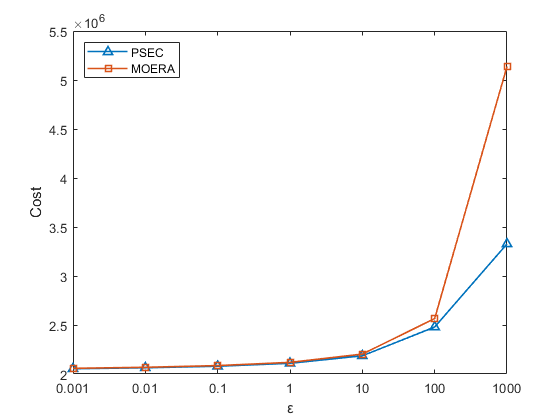
\includegraphics[width=2.9in,height=2.5in]{fig635.png} 
\centering
\fontsize{6.5}{8}\selectfont {\small{\textbf{Fig.8(a)}. The system cost versus  $\varepsilon $ }}
\end{minipage}
\begin{minipage}[t]{0.48\textwidth}
\centering
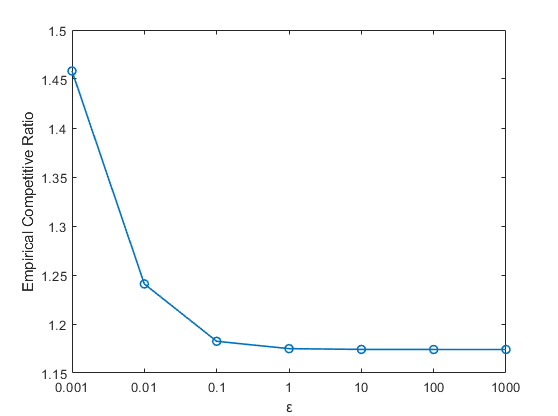
\includegraphics[width=2.9in,height=2.5in]{fig637.png} 
\centering
\fontsize{6.5}{8}\selectfont {\small{\textbf{Fig.8(b)}. The competitive ratio versus $\varepsilon $ of PSEC }}

\end{minipage}
\fontsize{6.5}{8}\selectfont {\small{\textbf{Fig.8}. The system performance versus $\varepsilon $ }}
\end{figure}





Fig.9 plots the total cost of different schemes with the increasing task size.  Obviously, the proposed scheme  is superior to other schemes and the gain is up to $40\%$. When the task size increases from 64 to 2048Mb, the  cost of PSEC is always less than $2.5*10^6$, while the cost of MOERA increased to more than $16*10^7$.  When the amount of data is greater than 100, the cost of MOERA shows a very obvious increase. PSEC  can always maintain a relatively stable state in terms of cost with the increasing task size.  This is because the task can be migrated from one edge node to another. Our PSEC can always help users find the most suitable edge node  for offloading and obtain a convergent and stable cost.
\begin{figure}[H]
\centering
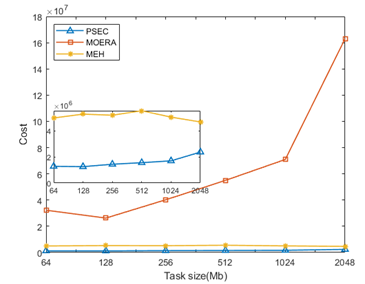
\includegraphics[width=3.2in,height=2.5in]{fig5.png} 
%\caption*{{\bf Fig.~4.}Divisible coin} \label{fig}

 \centering
\fontsize{6.5}{8}\selectfont {\small{\textbf{Fig.9}. The total cost versus the task size under different schemes}}
\end{figure}

%Fig. 10 illustrates the total cost of the three algorithms based on the change of   capacities.  We can discover that when the capacities becomes large, the total cost of the three algorithms also
%decreases.   This is because the more remaining capacity of edge nodes is, the stronger computing power is, and the better service can be provided for tasks. Although the PSEC method has less impact on the cost of %remaining node capacity than MEH method, and the difference is not obvious. As for various location-sensitive resource allocation problems, PSEC can still provide a more reliable service with a reasonable cost.
%\begin{figure}[H]
%\centering
%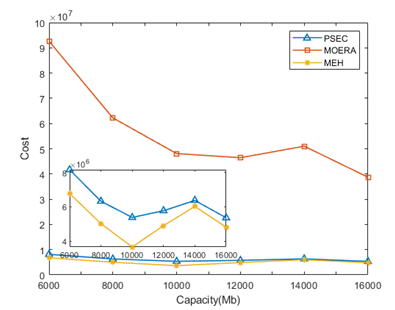
\includegraphics[width=3.2in,height=2.5in]{fig6.png} 
%%\caption*{{\bf Fig.~4.}Divisible coin} \label{fig}

 %\centering
%\fontsize{6.5}{8}\selectfont {\small{\textbf{Fig.10}. The total cost versus the capacity under different schemes}}
%\end{figure}



\section{Conclusion}
To solve the problem of task offloading in the resource-limited and position-sensitive multi-UAVs edge environment, a distributed location-aware task offloading  scheme based on convex optimal analysis is proposed. Considering the limited energy of edge nodes and the random movement of users, the total cost is divided into operation cost, quality of service cost, and migration cost. A nonlinear cost optimization problem is constructed, and then the problem is transformed into a convex optimization problem with linear constraints based on regularization technology. The mathematical proof shows that the scheme can support a parameterized competitive ratio without prior knowledge of the input task. Experimental results show that the proposed scheme can achieve  better performance with strong robustness.


%%%%%%%%%%%%%%%%%%%%%%%%%%%%%%%%%%%%%%%%%%
\vspace{6pt} 

%%%%%%%%%%%%%%%%%%%%%%%%%%%%%%%%%%%%%%%%%%
%% optional
%\supplementary{The following supporting information can be downloaded at:  \linksupplementary{s1}, Figure S1: title; Table S1: title; Video S1: title.}

% Only for the journal Methods and Protocols:
% If you wish to submit a video article, please do so with any other supplementary material.
% \supplementary{The following supporting information can be downloaded at: \linksupplementary{s1}, Figure S1: title; Table S1: title; Video S1: title. A supporting video article is available at doi: link.}

%%%%%%%%%%%%%%%%%%%%%%%%%%%%%%%%%%%%%%%%%%
\authorcontributions{Conceptualization, Jianhua Liu and Zibo Wu; Data curation, Xiaoguang Tu; Formal analysis, Zibo Wu; Funding acquisition,Jianhua Liu; Methodology, Jianhua Liu and Zibo Wu; Software, Xiaoguang Tu and Jiajia Liu; Supervision, Jianhua Liu; Writing—original draft, Jianhua Liu ; Writing—review and editing, Zibo Wu,Jiajia Liu, and Xiaoguang Tu. All authors have read and agreed tothe published version of the manuscript.}

\funding{This research was funded by College Students Innovation and Entrepreneurship Training Program No.S202110624133 and in part by the Civil Aviation Education Talent project under grant E2020014 .}





\conflictsofinterest{We authors declare no conflict of interest.} 

\textbf{Appendix A}\\
This appendix illustrates  the monotonicity proof of the competitive ratio.

Proof. We first review the following definitions:\\

\begin{align*}
r&=1+\gamma n_0,\\
\gamma&=max\{\left(z_s+\varepsilon\right)\eta_s\},\\
\eta_s&=\ln{\left(1+z_s/\varepsilon\right)},\\
z_s&=min\{Q_s/k,C_s\}
\end{align*}
To analysis the monotonicity competitive ratio $r$, we need to analyze  $\gamma$  which is related to the $\varepsilon$ as well as $z_s$. For above equations, $z_s$ is the minimum value of the array $\{Q_s/k,C_s\}$. Thus, a constant $z_0$ is existed which  is defined by the following formula:\\



\begin{equation*}
z_0= \mathop{\arg \max_{z_s}} \gamma \nonumber.
\end{equation*}


 Then, we have

\begin{equation*}
\gamma=\left(z_s+\varepsilon\right)\eta_s=\left(z_0+\varepsilon\right)\ln{\left(1+z_0/\varepsilon\right)},
\end{equation*}

and
\begin{equation*}
\gamma^{`}=\ln{\left(1+z_0/\varepsilon\right)}+\left(z_0+\varepsilon\right)\frac{-z_0\frac{1}{\varepsilon^2}}{1+\frac{z_0}{\varepsilon}}=\ln{\left(1+z_0/\varepsilon \right)}-\frac{z_0}{\varepsilon}=\ln{\left(1+z_0'\right)}-z_0',
\end{equation*}

where, $z_0'=\frac{z_0}{\varepsilon}$  and $\varepsilon$ is a positive number. According to the Taylor formula: $\ \ln{\left(1+x\right)}=x-\frac{x^2}{2}+\frac{x^3}{3}\ldots$, we have\\

\begin{equation*}
\ln{\left(1+z_0'\right)}-z_0'\le0,\quad z_0'>0.
\end{equation*}

Therefore, we can get
\begin{equation*}
\gamma^`=\ln{\left(1+z_0/\varepsilon\right)}-\frac{z_0}{\varepsilon}<0.
\end{equation*}

That is to say $\gamma$ is a subtractive function of $\varepsilon$, and we can get that the  competitive ratio $r$ decreases with the increase of $\varepsilon$.$\square$\\




%%%%%%%%%%%%%%%%%%%%%%%%%%%%%%%%%%%%%%%%%%
\begin{adjustwidth}{-\extralength}{0cm}
%\printendnotes[custom] % Un-comment to print a list of endnotes

\reftitle{References}

% Please provide either the correct journal abbreviation (e.g. according to the “List of Title Word Abbreviations” http://www.issn.org/services/online-services/access-to-the-ltwa/) or the full name of the journal.
% Citations and References in Supplementary files are permitted provided that they also appear in the reference list here. 

%=====================================
% References, variant A: external bibliography
%=====================================
%\bibliography{your_external_BibTeX_file}

%=====================================
% References, variant B: internal bibliography
%=====================================
\begin{thebibliography}{999}

\bibitem{Shenshihao20}
Shen,S.; Han, Y.; Wang, X.; Wang, Y. Computation Offloading with Multiple Agents in  Edge-Computing–Supported IoT. \emph{ACM Trans. Sens. Netw.} \textbf{2020}, \emph{16}, 1--27.

%2
\bibitem{Salaht20}
Salaht, F.; Desprez, F.; Lebre, A. An Overview of Service Placement Problem in Fog and Edge Computing. \emph{ACM Comput. Surv.} \textbf{2020}, \emph{53}, 1--35.
%3
\bibitem{ShiWeisong16}
Shi, W.; Cao, J.; Zhang, Q.; Li, Y.; Xu, L. Edge Computing: Vision and Challenges. \emph{IEEE Internet Things J.} \textbf{2016}, \emph{3}, 637--646.

\bibitem{Liuyaqiong20}
Liu, Y.; Peng, M.; Shou, G.; Chen, Y.; Chen, S. Toward Edge Intelligence: Multiaccess Edge Computing for 5G and Internet of Things. \emph{IEEE Internet Things J.} \textbf{2020}, \emph{7}, 6722--6747.

\bibitem{YuyiMao2016}
Mao, Y.; Zhang, J.; Letaief, K. Dynamic Computation Offloading for Mobile-Edge Computing With Energy Harvesting Devices. \emph{IEEE J. Sel. Areas Commun.} \textbf{2016}, \emph{34}, 3590--3605.
% Reference 1
\bibitem{Faraci20}
Faraci, G. Grasso, C. Schembra, G. Fog in the Clouds: UAVs to Provide Edge Computing to IoT Devices. \emph{ACM Transactions on Internet Technology}. \textbf{2020}, \emph{3},1--26.
\bibitem{XuY21}
Xu, Y.; Zhang, T.; Loo, J., et al. Completion time minimization for UAV-assisted mobile-edge computing systems. \emph{ IEEE Transactions on Vehicular Technology.} \emph{2021}, \emph{11}, 12253--12259.
\bibitem{WangH19}
Wang, H.; Wang, J. ; Ding, G. ; Chen, J.; Gao, F.;and Han, Z. Completion time minimization with path planning for fixed-wing UAV communications. \emph{IEEE Trans. Wireless Commun.}, \textbf{2019}, \emph{7}, 3485--3499.
\bibitem{ZhanC19}
Zhan, C. ; Zeng, Y.  Completion time minimization for multi-UAVenabled data collection.  \emph{IEEE Trans. Wireless Commun.}, \textbf{2019}, \emph{10}, 4859--4872. 
\bibitem{ZengY18}
Zeng, Y.; Xu, X.; and Zhang, R. Trajectory design for completion time minimization in UAV-enabled multicasting. \emph{IEEE Trans. Wireless Commun.}  \textbf{2018}, \emph{4}, 2233—2246. 

\bibitem{Wangtian19}
Wang, T.; Zhang, G.; Liu, A.; Bhuiyan, A.; Jin, Q. A Secure IoT Service Architecture with an Efficient Balance Dynamics Based on Cloud and Edge Computing. \emph{IEEE Internet Thing J.} \textbf{2019}, \emph{6}, 4831--4843.
\bibitem{Satyanarayanan17}
Satyanarayanan, M. The emergence of edge computing. \emph{Computer}, \emph{2017}, \emph{1},  30--39.
\bibitem{WANG}
Wang,L; Lei, J; Li,J.  MOERA: Mobility-agnostic Online Resource Allocation for Edge Computing . \emph{IEEE Transactions on Mobile Computing},\textbf{2019},\emph{9},1843--1856. 


\bibitem{WU Q}
	Wu,Q.; Me,W.;Zhang,R. Safeguarding wireless network with UAVs: a physical layer security perspective . \emph{IEEE Wireless Communications},\textbf{2019},\emph{26},12--18.
% Reference 2
\bibitem{CUI G F}
Cui,G.;Xu,Y; Zhang,S; WANG,W. Secure data offloading strategy for multi-UAV wireless networks based on minimum energy consumption. \emph{Journal on Communications}. May.,2021,vol.42,pp.51--62.
% Reference 3
\bibitem{JI J}
Ji,J;Zhu,K; Yi,C. Energy Consumption Minimization in UAV-Assisted Mobile-Edge Computing Systems: Joint Resource Allocation and Trajectory Design. \emph{IEEE Inter-net of Things Journal},\textbf{2021},\emph{8},8570-–8584.
% Reference 4
\bibitem{WANG Y P}
Wang,Y;Fang,W;Ding,Y; Xiong,N. Computation offloading optimization for UAV-assisted mobile edge computing: a deep deterministic policy gradient ap-proach.\emph{Wireless Networks},\textbf{2021},\emph{27},2991–-3006.
% Reference 5
\bibitem{GOPIKA P}
Gopika,P;Mario,D;Tarik,T. Edge Computing for the Internet of Things: A Case Study .\emph{ IEEE Internet of Things Journal},\textbf{2018},\emph{5},1275--1284.
% Reference 6
\bibitem{PAN J L}
Pan,J; Mcelhannon,J. Future Edge Cloud and Edge Computing for Internet of Things Applications . \emph{IEEE Internet of Things Journal}, \textbf{2018},\emph{5},439--449.
% Reference 7
\bibitem{ZHANG K Y}
Zhang,K; Lin,G; Wang,R; Jing,L; Sheng,R. Survey on computation offloading and content caching in mobile edge networks. \emph{Journal of Software},\textbf{2019}, \emph{30},2491--2516.
% Reference 8
\bibitem{ZHANG N}
Zhang,N; Guo,S; Dong,Y; Liu,D. Joint task offloading and data caching in mobile edge computing net-works . \emph{Computer Networks},\textbf{2020},\emph{182},107446.
% Reference 9
\bibitem{WANG S}
Wang,S; Chen,M; Liu,X. A Machine Learning Approach for Task and Resource Allocation in Mobile Edge Computing Based Networks . \emph{IEEE Internet of Things Journal}, \textbf{2020},\emph{182},6824--6836.
% Reference 10
\bibitem{LIU}
Liu,Y; Peng,M; Shou,G; Chen,Y; Chen,S. Toward Edge Intelligence: Multi-access Edge Computing for 5G and Internet of Things.\emph{ IEEE Internet of Things Journal},\textbf{2020},\emph{7},6722--6747.
% Reference 1

% Reference 2
\bibitem{HABER}
Haber,E ; Nguyen, T ; Assi,C. An ener-gy-efficient task offloading solution for MEC-based IoT in Ultra-dense networks\emph{2019 IEEE Wireless Communi-cations and Networking Conference. Piscataway: IEEE Press}, 2019, 1--7.
% Reference 3
\bibitem{CHEN M}
Chen, M; Hao,Y. Task Offloading for Mobile Edge Computing in Software Defined Ultra-dense Network. \emph{IEEE Journal on Selected Areas in Communications}.\textbf{2018},36,587--597. 
% Reference 4
\bibitem{PUTHAL}
Puthal,D; Obaidat,M;Nanda,P; Prasad,M. MOHANTY S P, ZOMAYA A Y.Secure and Sustainable Load Balancing of Edge Data Centers in Fog Computing . \emph{IEEE Communications Magazine},\textbf{2018},56,60--65.
% Reference 5
\bibitem{XU X L}
Xu ,X; Wu, Q; Dou,W; Tsai,S. Trust-Aware Service Offloading for Video Surveillance in Edge Compu-ting Enabled Internet of Vehicles. \emph{IEEE transactions on intelligent transportation systems},\textbf{2021},22,1787--1796.
% Reference 6


\bibitem{Zhusc20}
Zhu, S.; Gui, L..; Cheng, N.; Zhang, Q.; Sun, F.; and Lang, X. UAV-enabled computation migration for complex missions: A reinforcement learning approach.  \emph{IET Communications.}  \textbf{2020},  \emph{15}, 2472--2480.
\bibitem{Callegaro2021}
Callegaro, D.; Levorato, M. Optimal edge computing for infrastructure-assisted uav systems.  \emph{IEEE Transactions on Vehicular Technology}, \textbf{2021},  \emph{2},  1782--1792.
\bibitem{Amos2021}
Amos, P.; Li, P.; Wu, W.; Wang, B. Computation efficiency maximization for secure UAV-enabled mobile edge computing networks.  \emph{Physical Communication}, \textbf{2021},  \emph{46}, 101284.

\bibitem{RuiHan2020}
Han, R.; Wen, Y.; Bai, L.; Liu, J.; and  Choi, J. Rate splitting on mobile edge computing for UAV-aided IoT systems. \emph{IEEE Transactions on Cognitive Communications and Networking},  \textbf{2020}, \emph{4}, 1193--1203.


\bibitem{WangX2020}
Wang, X.; Ning, Z.; Guo, S. Multi-agent imitation learning for pervasive edge computing: a decentralized computation offloading algorithm. \emph{IEEE Transactions on Parallel and Distributed Systems}, \textbf{2021}, \emph{2}, 411--425.
\bibitem{Thomas2020}
Thomas; Marlin, U. Queueing systems. \emph{SIAM Rev.} \textbf{1977}, \emph{3},
 512--514.
\bibitem{Bubeck2015}
Bubeck, S. Convex optimization: Algorithms and complexity.
\emph{Found. Trends Mach. Learn.} \textbf{2015}, \emph{3/4},231--257.
\bibitem{LiW21}
LI, W.; JIN, S.Performance evaluation and optimization of a task offloading strategy on the mobile edge computing with edge heterogeneity. \emph{The Journal of Supercomputing}, \textbf{2021},\emph{11},12486--12507.

\end{thebibliography}

% If authors have biography, please use the format below
%\section*{Short Biography of Authors}
%\bio
%{\raisebox{-0.35cm}{\includegraphics[width=3.5cm,height=5.3cm,clip,keepaspectratio]{Definitions/author1.pdf}}}
%{\textbf{Firstname Lastname} Biography of first author}
%
%\bio
%{\raisebox{-0.35cm}{\includegraphics[width=3.5cm,height=5.3cm,clip,keepaspectratio]{Definitions/author2.jpg}}}
%{\textbf{Firstname Lastname} Biography of second author}

% For the MDPI journals use author-date citation, please follow the formatting guidelines on http://www.mdpi.com/authors/references
% To cite two works by the same author: \citeauthor{ref-journal-1a} (\citeyear{ref-journal-1a}, \citeyear{ref-journal-1b}). This produces: Whittaker (1967, 1975)
% To cite two works by the same author with specific pages: \citeauthor{ref-journal-3a} (\citeyear{ref-journal-3a}, p. 328; \citeyear{ref-journal-3b}, p.475). This produces: Wong (1999, p. 328; 2000, p. 475)

%%%%%%%%%%%%%%%%%%%%%%%%%%%%%%%%%%%%%%%%%%
%% for journal Sci
%\reviewreports{\\
%Reviewer 1 comments and authors’ response\\
%Reviewer 2 comments and authors’ response\\
%Reviewer 3 comments and authors’ response
%}
%%%%%%%%%%%%%%%%%%%%%%%%%%%%%%%%%%%%%%%%%%
\end{adjustwidth}
\end{document}

